\documentclass[UTF8,a4paper,12pt]{ctexart}

\usepackage{geometry}
\usepackage{graphicx}
\usepackage{booktabs}
\usepackage{float}
\usepackage{hyperref}
\usepackage{verbatim}
\usepackage{listings}
\usepackage{xcolor}
\usepackage{array}
\usepackage{caption}
\usepackage{subcaption}

\geometry{left=2.5cm,right=2.5cm,top=2.5cm,bottom=2.5cm}

% 代码高亮设置
\definecolor{codegreen}{rgb}{0,0.6,0}
\definecolor{codegray}{rgb}{0.5,0.5,0.5}
\definecolor{codepurple}{rgb}{0.58,0,0.82}
\definecolor{backcolour}{rgb}{0.95,0.95,0.92}
\definecolor{highlightbg}{rgb}{0.85,0.95,0.85}

\lstdefinestyle{mystyle}{
    backgroundcolor=\color{backcolour},
    commentstyle=\color{codegreen},
    keywordstyle=\color{magenta},
    numberstyle=\tiny\color{codegray},
    stringstyle=\color{codepurple},
    basicstyle=\ttfamily\small,
    breakatwhitespace=false,
    breaklines=true,
    captionpos=b,
    keepspaces=true,
    numbers=left,
    numbersep=5pt,
    showspaces=false,
    showstringspaces=false,
    showtabs=false,
    tabsize=2
}
\lstset{style=mystyle}

\title{基于卷积神经网络的 MNIST 手写数字识别实验报告}
\author{姓名：\underline{刘泽睿} \quad 学号：\underline{PB24000157}}
\date{\today}

\begin{document}

\maketitle

\begin{abstract}
本实验基于卷积神经网络对 MNIST 手写数字数据集进行分类任务。
实验对比了两种不同深度的卷积网络架构（双卷积层的基础结构与引入批量归一化的五卷积层深层结构），
并在学习率、权重衰减、丢弃率三个超参数构成的 $2\times2\times2$ 网格上进行了系统性搜索，
共计 16 组对照实验。实验结果表明，深层网络在最佳超参数配置下取得了
\textbf{99.57\%} 的测试准确率，显著优于基础网络的最佳结果 \textbf{99.37\%}。
本文完整记录了实验设计、模型架构、超参数配置、实验结果与分析，以及调试过程。
完整代码已开源至 \url{https://github.com/mathmonkeyliu/USTC-AI-homework}。
\end{abstract}

\tableofcontents

\section{引言}

手写数字识别是计算机视觉领域的经典入门任务，是模式分类中的基础问题。
MNIST 数据集包含 60,000 张训练图像和 10,000 张测试图像，每张为 $28\times28$ 的灰度手写数字图像，
共 10 个类别（0--9）。卷积神经网络因其在图像特征提取上的优异表现，
已成为 MNIST 任务上的标准方法。

本实验旨在探究不同网络深度及超参数设置对手写数字识别性能的影响。
实验对比了两种模型结构：一种为仅含两个卷积层的基础网络，
另一种为引入批量归一化的五卷积层深层网络。
此外，实验在三个关键超参数上进行了网格搜索——学习率、权重衰减系数和丢弃率，
以探索各超参数对模型性能的影响规律。

\section{实验设计}

\subsection{数据集}

实验使用 MNIST 手写数字数据集，包含 60,000 张训练图像和 10,000 张测试图像。
每张图像为 $28\times28$ 像素的单通道灰度图。数据预处理流程如下：
\begin{enumerate}
    \item 将 PIL 图像转换为 PyTorch Tensor（\texttt{transforms.ToTensor()}）；
    \item 使用 MNIST 数据集的全局均值和标准差进行归一化：\texttt{Normalize((0.1307,), (0.3081,))}。
\end{enumerate}

训练时以每批 64 张图像加载数据并随机打乱，测试时不打乱。

\subsection{模型架构}

实验实现了两种卷积神经网络，二者的核心差异在于网络深度和是否使用批量归一化。

\subsubsection{基础 CNN：双卷积层结构}

基础网络由一个简单的特征提取器和一个分类器组成，结构如下：

\begin{itemize}
    \item \textbf{特征提取器}：两层卷积，每层后接 ReLU 激活和 $2\times2$ 最大池化：
    \begin{verbatim}
    Conv2d(1, 32, 3×3, padding=1) → ReLU → MaxPool2d(2)  # 28→14
    Conv2d(32, 64, 3×3, padding=1) → ReLU → MaxPool2d(2)  # 14→7
    \end{verbatim}
    \item \textbf{分类器}：全连接层：
    \begin{verbatim}
    Flatten → Linear(64×7×7, 128) → ReLU → Dropout(p) → Linear(128, 10)
    \end{verbatim}
\end{itemize}

该模型参数量约为 0.42M。

\subsubsection{深层 CNN：五卷积层 + 批量归一化结构}

深层网络在基础网络之上进行了三方面增强：增加卷积层数、引入批量归一化层、扩展通道数与全连接层宽度。
该模型由三个卷积块组成：

\begin{itemize}
    \item \textbf{卷积块一}（双层卷积 + 批量归一化）：
    \begin{verbatim}
    Conv2d(1, 32, 3×3) → BN → ReLU
    Conv2d(32, 32, 3×3) → BN → ReLU → MaxPool2d(2)  # 28→14
    \end{verbatim}
    \item \textbf{卷积块二}（双层卷积 + 批量归一化）：
    \begin{verbatim}
    Conv2d(32, 64, 3×3) → BN → ReLU
    Conv2d(64, 64, 3×3) → BN → ReLU → MaxPool2d(2)  # 14→7
    \end{verbatim}
    \item \textbf{卷积块三}（单层卷积 + 批量归一化）：
    \begin{verbatim}
    Conv2d(64, 128, 3×3) → BN → ReLU → MaxPool2d(2)  # 7→3
    \end{verbatim}
    \item \textbf{分类器}：
    \begin{verbatim}
    Flatten → Linear(128×3×3, 256) → ReLU → Dropout(p) → Linear(256, 10)
    \end{verbatim}
\end{itemize}

该模型参数量约为 0.55M。

\subsection{架构差异分析}

相比于基础网络，深层网络从以下几个方面进行了增强：

\begin{enumerate}
    \item \textbf{增加网络深度}：基础网络仅有 2 个卷积层，而深层网络提升至 5 个卷积层（分布在三个卷积块中），
          显著增强了模型的特征提取能力；
    \item \textbf{引入批量归一化}：在每个卷积层后添加批量归一化层，
          有效缓解了内部协变量偏移问题，加速收敛并提升训练稳定性；
    \item \textbf{扩展卷积通道数}：基础网络的通道数从 32 递增至 64，而深层网络扩展至 $32 \to 64 \to 128$，
          更宽的通道数使模型能捕捉更丰富的特征表示；
    \item \textbf{扩大全连接隐藏层}：分类器的隐藏层维度从 128 提升至 256，
          增强了分类头的非线性表达能力。
\end{enumerate}

这些修改使深层网络具备了更强的表征能力。得益于批量归一化层的引入，
深层网络在训练过程中收敛更快、更稳定，且最终取得了明显更高的测试准确率。

\subsection{超参数搜索空间}

实验对三个关键超参数进行网格搜索，每个超参数设两个取值，构成 $2\times2\times2=8$ 种组合：

\begin{itemize}
    \item 学习率：$\{0.0005,\; 0.001\}$
    \item 权重衰减系数：$\{0.0,\; 0.0001\}$
    \item 丢弃率：$\{0.3,\; 0.5\}$
\end{itemize}

\subsection{训练配置}

所有实验共享以下固定配置：

\begin{itemize}
    \item 优化器：Adam
    \item 损失函数：交叉熵损失
    \item 训练轮数：10
    \item 批次大小：64
    \item 随机种子：42
    \item 数据加载工作进程数：2
    \item 日志记录间隔：每 100 个批次
\end{itemize}

上述 8 种超参数组合分别在两种模型上训练，共计 16 组实验。

\section{实验结果与分析}

\subsection{总体结果}

表~\ref{tab:results} 展示了所有 16 组实验在 MNIST 测试集上的最佳准确率。
每列最优结果已加粗标出。

\begin{table}[H]
\centering
\caption{不同超参数配置与模型组合下的测试集最佳准确率}
\label{tab:results}
\begin{tabular}{ccccc>{\bfseries}cc}
\toprule
\textbf{编号} & \textbf{学习率} & \textbf{权重衰减} & \textbf{丢弃率} & \textbf{基础 CNN} & \textbf{深层 CNN} \\
\midrule
1 & 0.0005 & 0.0    & 0.3 & 0.9927 & \textbf{0.9957} \\
2 & 0.0005 & 0.0001 & 0.3 & 0.9933 & 0.9948 \\
3 & 0.001  & 0.0    & 0.3 & 0.9932 & 0.9951 \\
4 & 0.001  & 0.0001 & 0.3 & 0.9925 & 0.9952 \\
5 & 0.0005 & 0.0    & 0.5 & \textbf{0.9937} & \textbf{0.9957} \\
6 & 0.0005 & 0.0001 & 0.5 & 0.9926 & 0.9951 \\
7 & 0.001  & 0.0    & 0.5 & 0.9932 & 0.9947 \\
8 & 0.001  & 0.0001 & 0.5 & 0.9925 & 0.9940 \\
\midrule
\multicolumn{4}{c}{\textbf{基础 CNN 最佳}} & \textbf{0.9937} & --- \\
\multicolumn{4}{c}{\textbf{深层 CNN 最佳}} & --- & \textbf{0.9957} \\
\bottomrule
\end{tabular}
\end{table}

\subsection{结果分析}

\subsubsection{模型架构对性能的影响}

从表~\ref{tab:results} 可以清晰地看出，\textbf{深层网络在所有 8 组超参数配置下均优于基础网络}。
深层网络的最佳准确率为 0.9957，比基础网络的最佳准确率 0.9937 高出 0.20 个百分点。
考虑到 MNIST 数据集的准确率已经处于较高水平（$>99\%$），这一提升是显著的。

深层网络的性能优势主要来源于：
\begin{enumerate}
    \item \textbf{更深的网络结构}：5 个卷积层（相比之下基础网络仅 2 个）提供了更强的特征提取能力，能够学习更抽象、更具判别力的特征；
    \item \textbf{批量归一化}：使各层输入的分布更加稳定，允许使用更大的学习率并加速收敛，同时具有一定的正则化效果；
    \item \textbf{更宽的特征图}：通道数从基础网络的 64 扩展到 128，使模型能表示更丰富的视觉模式。
\end{enumerate}

\subsubsection{超参数对性能的影响}

对基础网络而言：
\begin{itemize}
    \item 较低的学习率（0.0005）整体表现优于较高的学习率（0.001），说明浅层网络对学习率更为敏感；
    \item 不使用权重衰减的配置普遍优于使用权重衰减（0.0001）的对应配置；
    \item 在学习率为 0.0005、不使用权重衰减的条件下，较高的丢弃率（0.5）取得了该模型的最佳结果（0.9937），而较低的丢弃率（0.3）则为 0.9927，差异不大。
\end{itemize}

对深层网络而言：
\begin{itemize}
    \item 模型对超参数变化表现出更强的鲁棒性：8 组配置的准确率波动范围为 0.9940--0.9957（极差 0.0017），
          而基础网络的波动范围为 0.9925--0.9937（极差 0.0012）；
    \item 不使用权重衰减时准确率普遍更高，说明批量归一化本身已提供足够的正则化效果，额外的权重衰减反而可能限制模型容量；
    \item 最优配置出现在学习率为 0.0005 且不使用权重衰减的条件下（表~\ref{tab:results} 中编号 1 与 5），
          两者均达到 0.9957，表明在该条件下深层网络对丢弃率（0.3 与 0.5）不敏感。
\end{itemize}

\subsection{训练过程准确率曲线}

图~\ref{fig:base_cnn_accuracy} 和图~\ref{fig:deep_cnn_accuracy} 分别展示了基础 CNN 和深层 CNN
在 8 组超参数配置下的训练与测试准确率随训练轮数的变化趋势。
图中曲线直接截取自 TensorBoard 可视化面板，
图例中的标签对应于不同超参数配置的实验运行名称，
其与表~\ref{tab:results} 中编号的对应关系及具体超参数取值见表~\ref{tab:legend_mapping}。

\begin{table}[H]
\centering
\caption{TensorBoard 图例标签与超参数配置的对应关系}
\label{tab:legend_mapping}
\begin{tabular}{cccc}
\toprule
\textbf{图例标签（基础 CNN）} & \textbf{图例标签（深层 CNN）} & \textbf{表~\ref{tab:results} 编号} & \textbf{超参数} \\
\midrule
config\_1\_model\_1 & config\_1\_model\_2 & 1 & lr=0.0005, wd=0.0, dropout=0.3 \\
config\_2\_model\_1 & config\_2\_model\_2 & 2 & lr=0.0005, wd=0.0001, dropout=0.3 \\
config\_3\_model\_1 & config\_3\_model\_2 & 3 & lr=0.001, wd=0.0, dropout=0.3 \\
config\_4\_model\_1 & config\_4\_model\_2 & 4 & lr=0.001, wd=0.0001, dropout=0.3 \\
config\_5\_model\_1 & config\_5\_model\_2 & 5 & lr=0.0005, wd=0.0, dropout=0.5 \\
config\_6\_model\_1 & config\_6\_model\_2 & 6 & lr=0.0005, wd=0.0001, dropout=0.5 \\
config\_7\_model\_1 & config\_7\_model\_2 & 7 & lr=0.001, wd=0.0, dropout=0.5 \\
config\_8\_model\_1 & config\_8\_model\_2 & 8 & lr=0.001, wd=0.0001, dropout=0.5 \\
\bottomrule
\end{tabular}
\end{table}

\begin{figure}[H]
    \centering
    \begin{subfigure}[b]{0.48\textwidth}
        \centering
        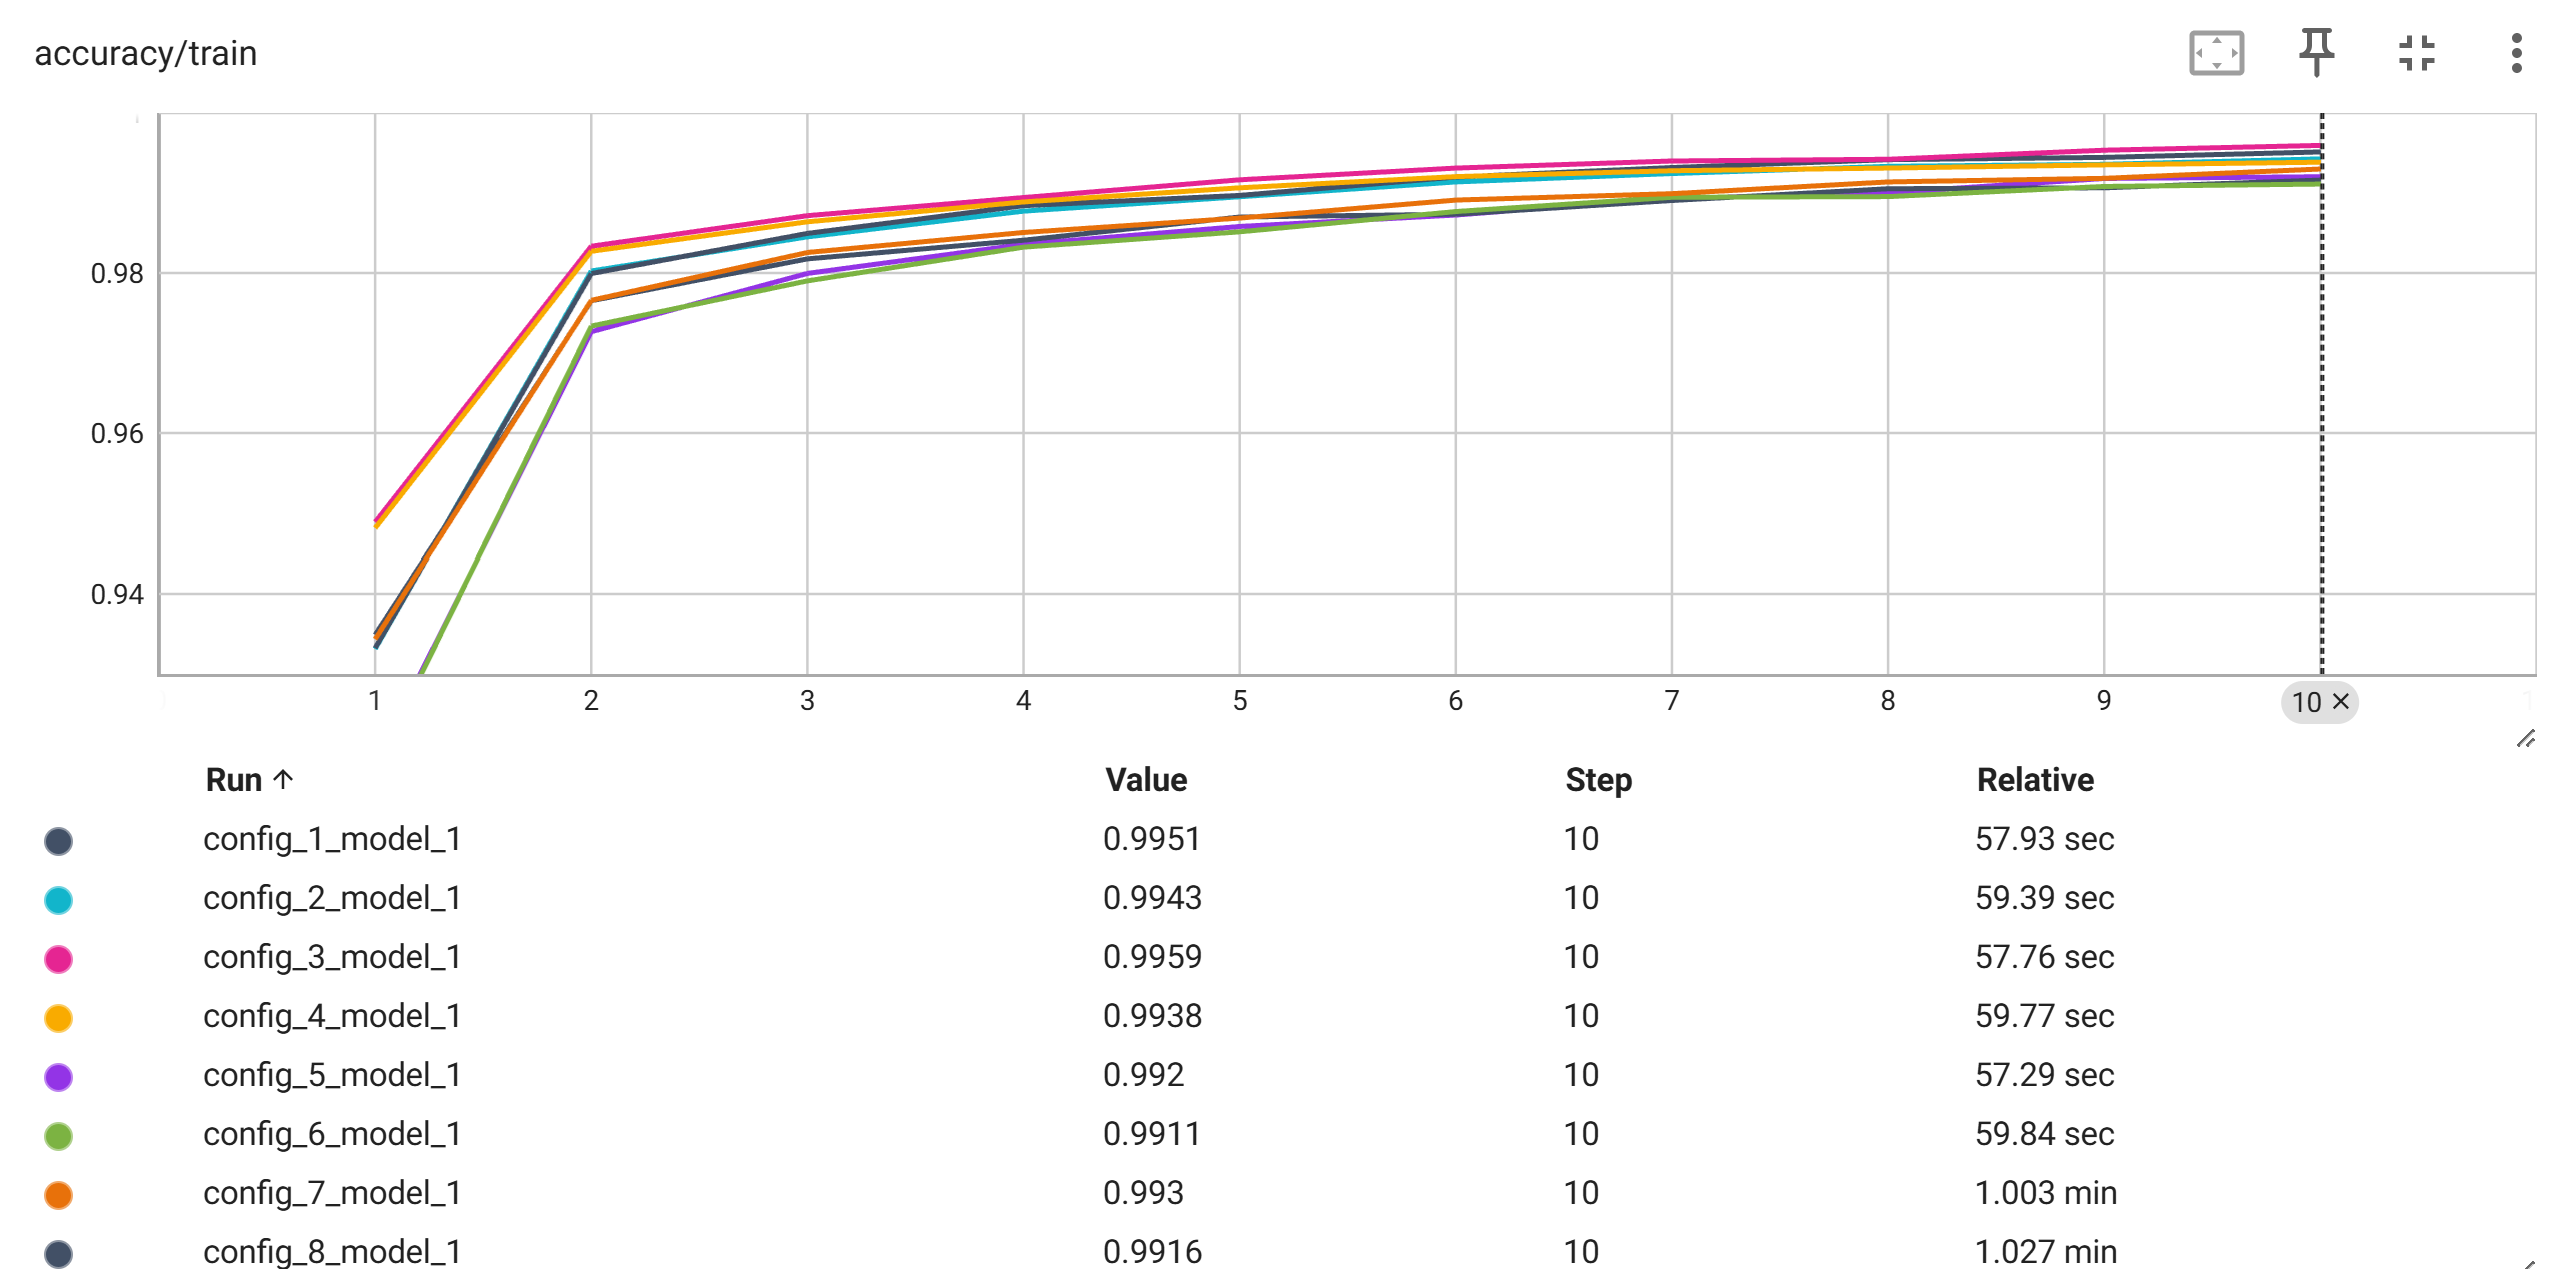
\includegraphics[width=\textwidth]{src/model_1_train_accurary.png}
        \caption{训练准确率}
        \label{fig:base_train_acc}
    \end{subfigure}
    \hfill
    \begin{subfigure}[b]{0.48\textwidth}
        \centering
        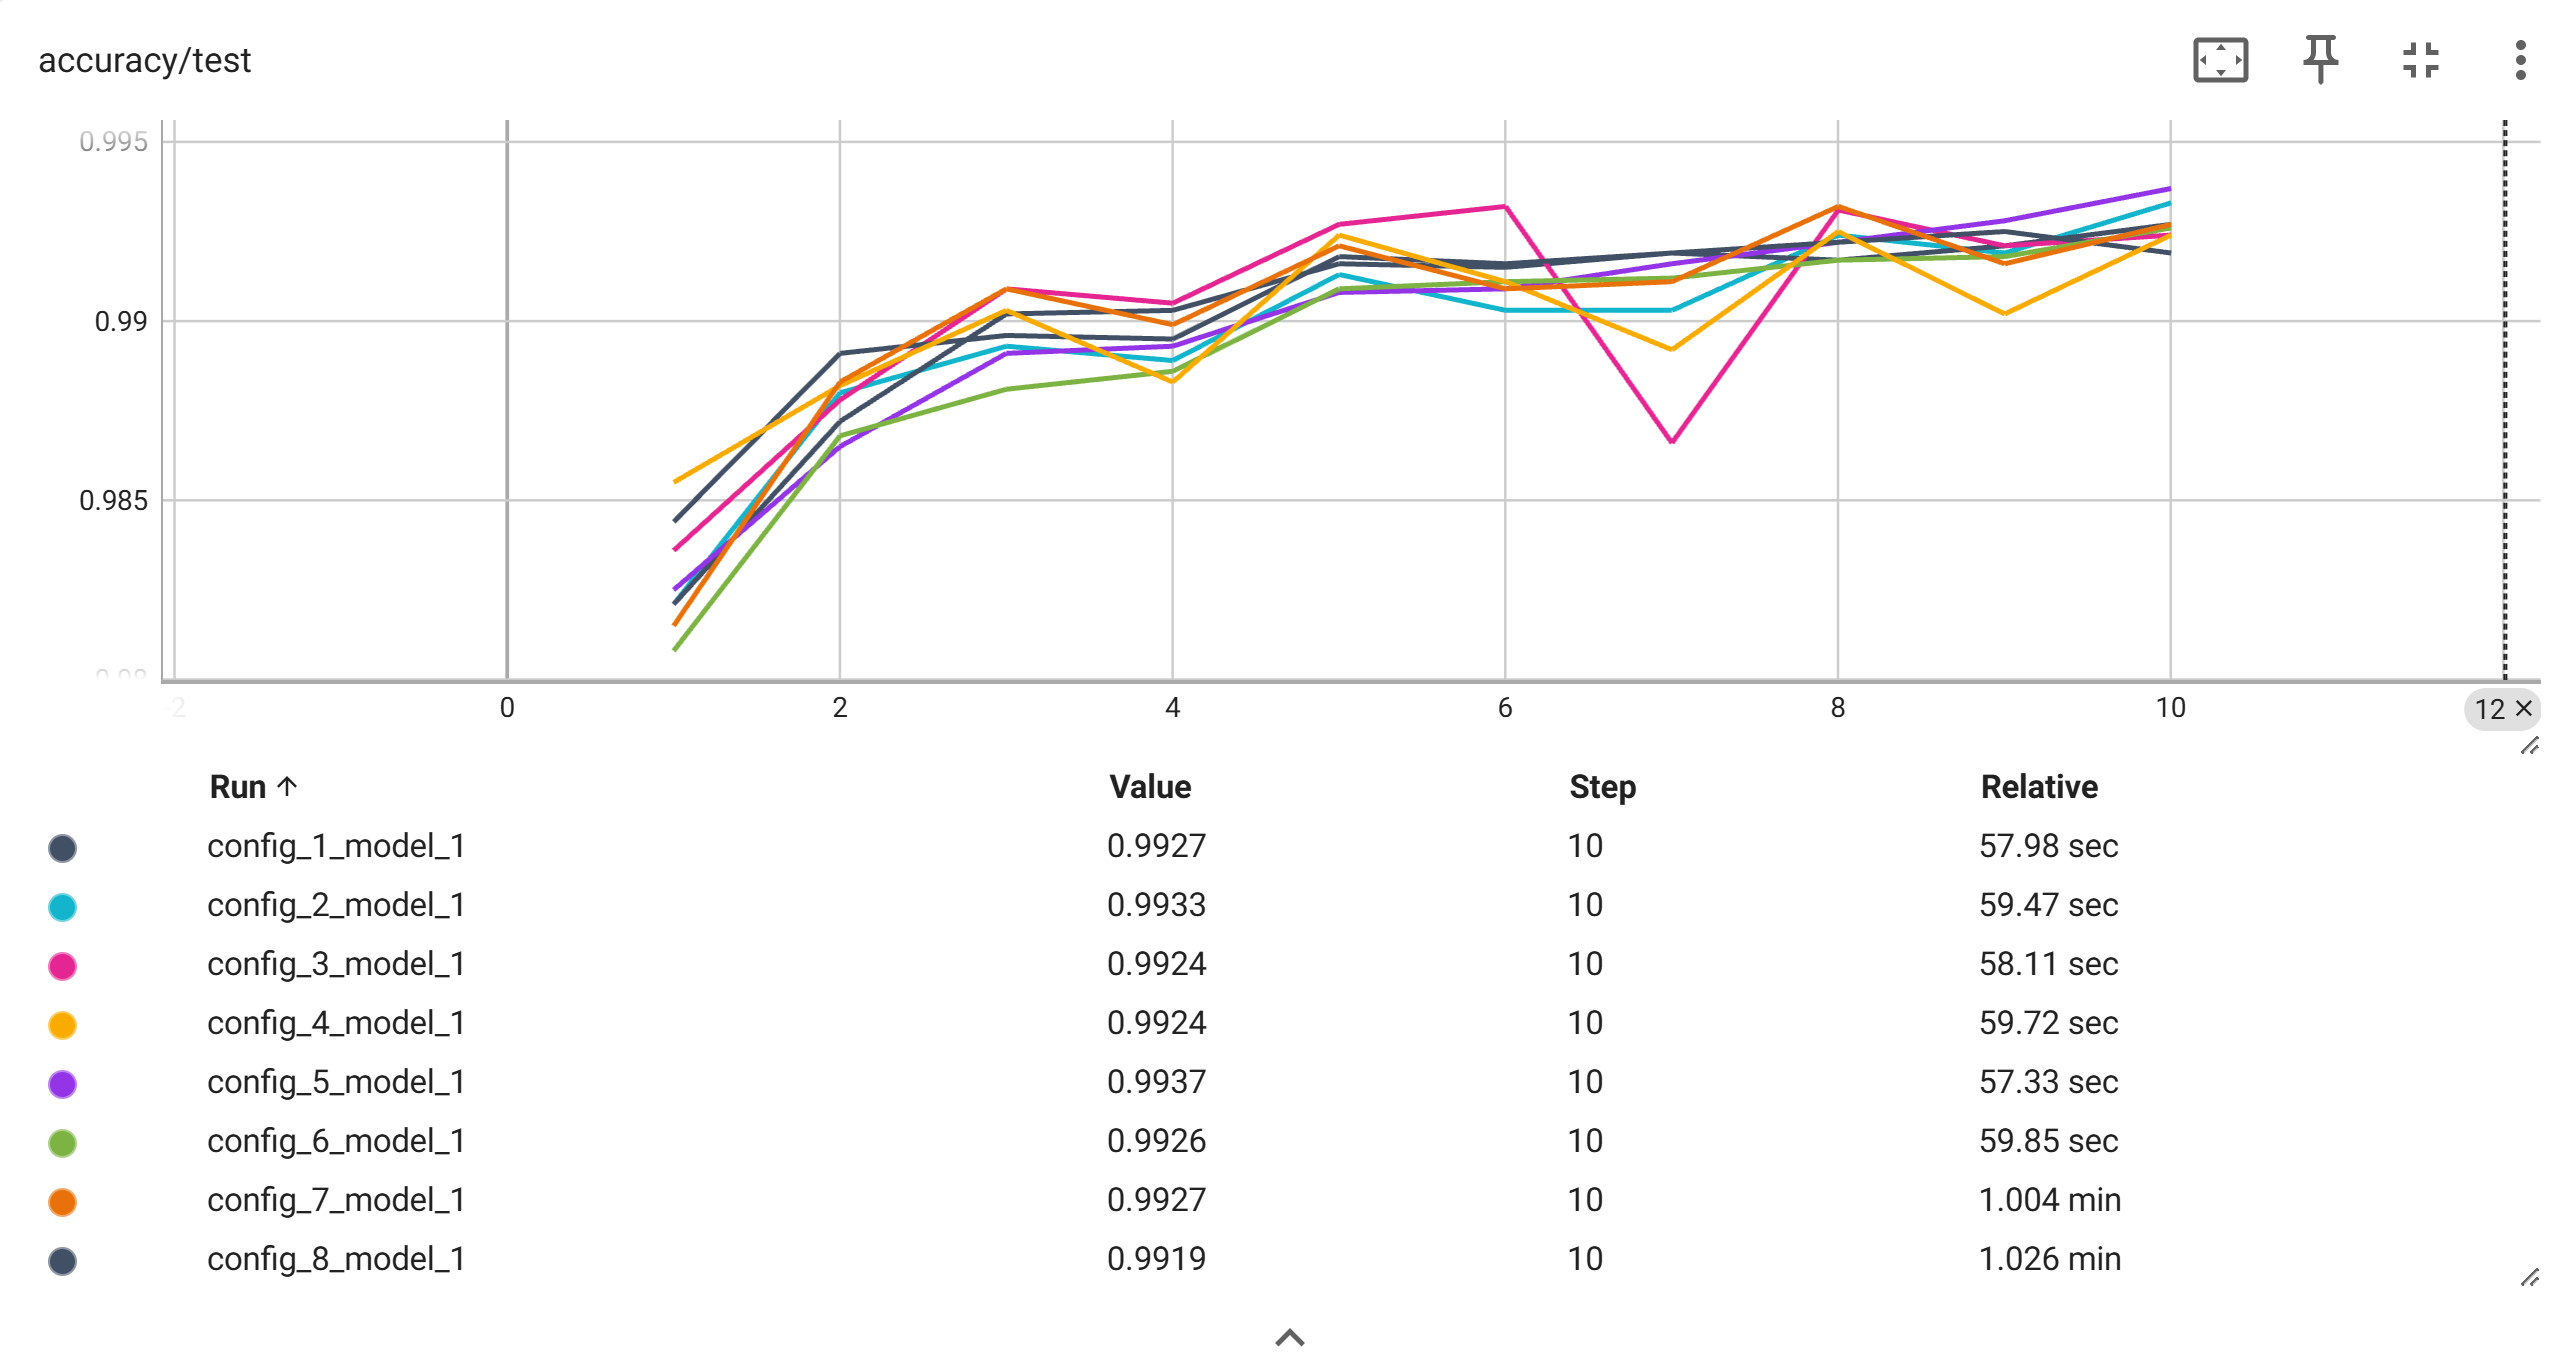
\includegraphics[width=\textwidth]{src/model_1_test_accurary.png}
        \caption{测试准确率}
        \label{fig:base_test_acc}
    \end{subfigure}
    \caption{基础 CNN（双卷积层结构）在 8 组超参数配置下的准确率曲线。
    图例标签与超参数配置的对应关系见表~\ref{tab:legend_mapping}。}
    \label{fig:base_cnn_accuracy}
\end{figure}

\begin{figure}[H]
    \centering
    \begin{subfigure}[b]{0.48\textwidth}
        \centering
        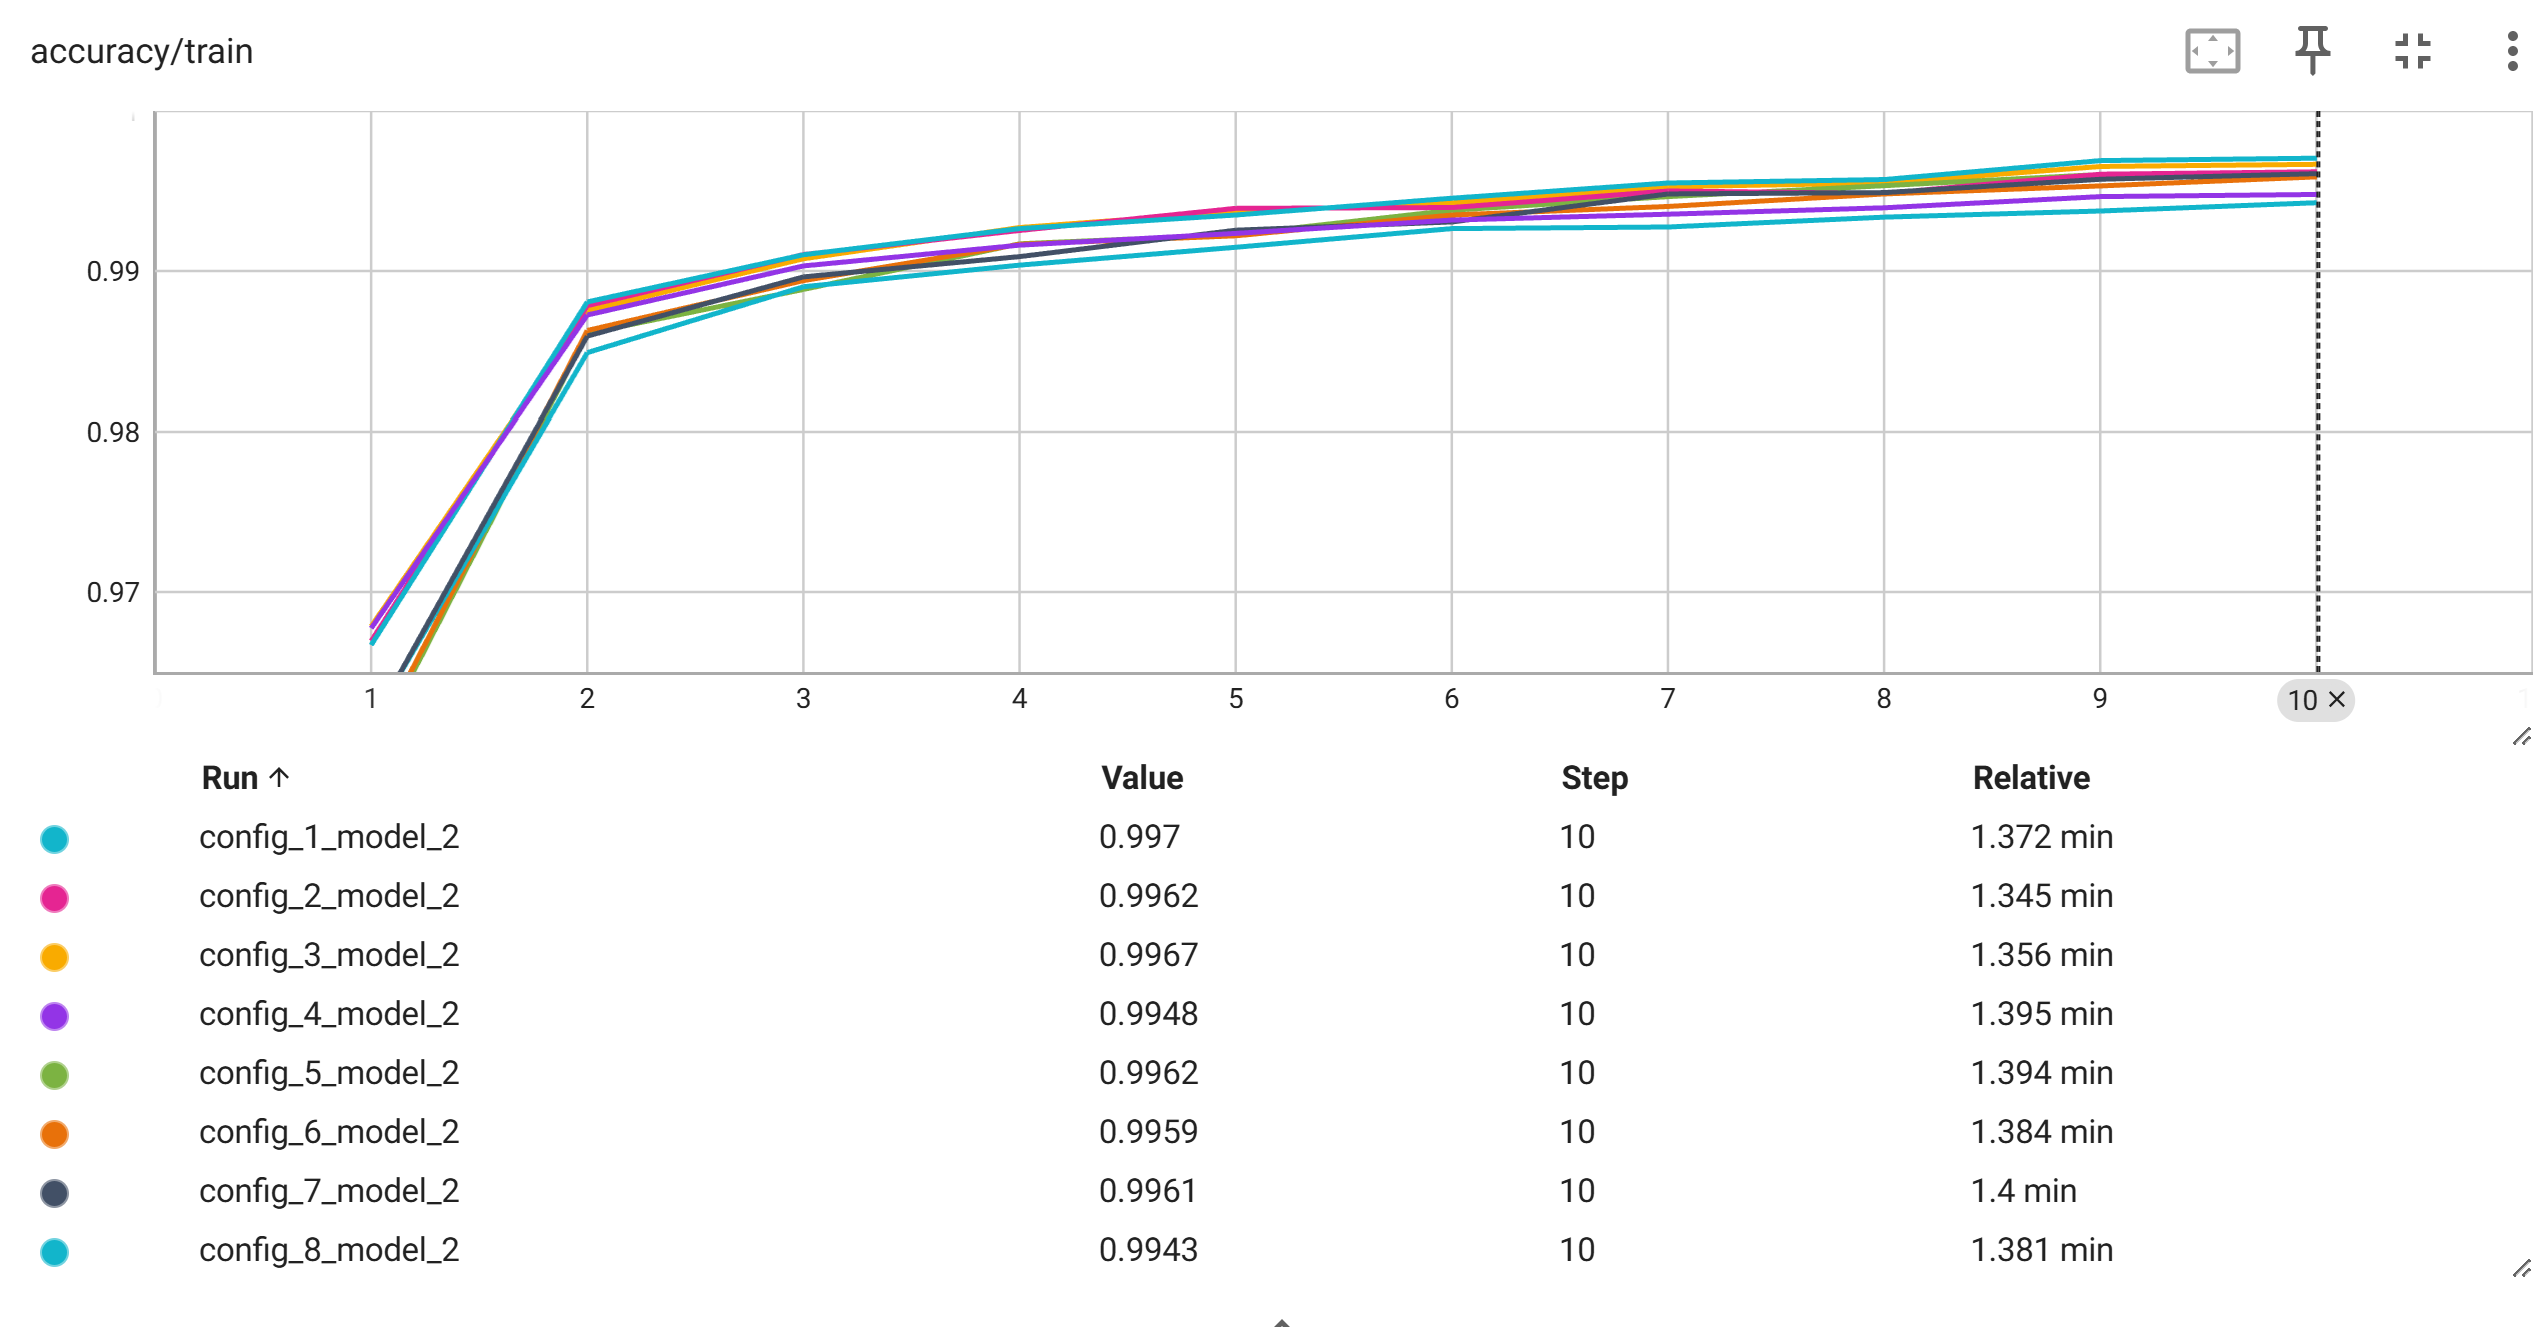
\includegraphics[width=\textwidth]{src/model_2_train_accurary.png}
        \caption{训练准确率}
        \label{fig:deep_train_acc}
    \end{subfigure}
    \hfill
    \begin{subfigure}[b]{0.48\textwidth}
        \centering
        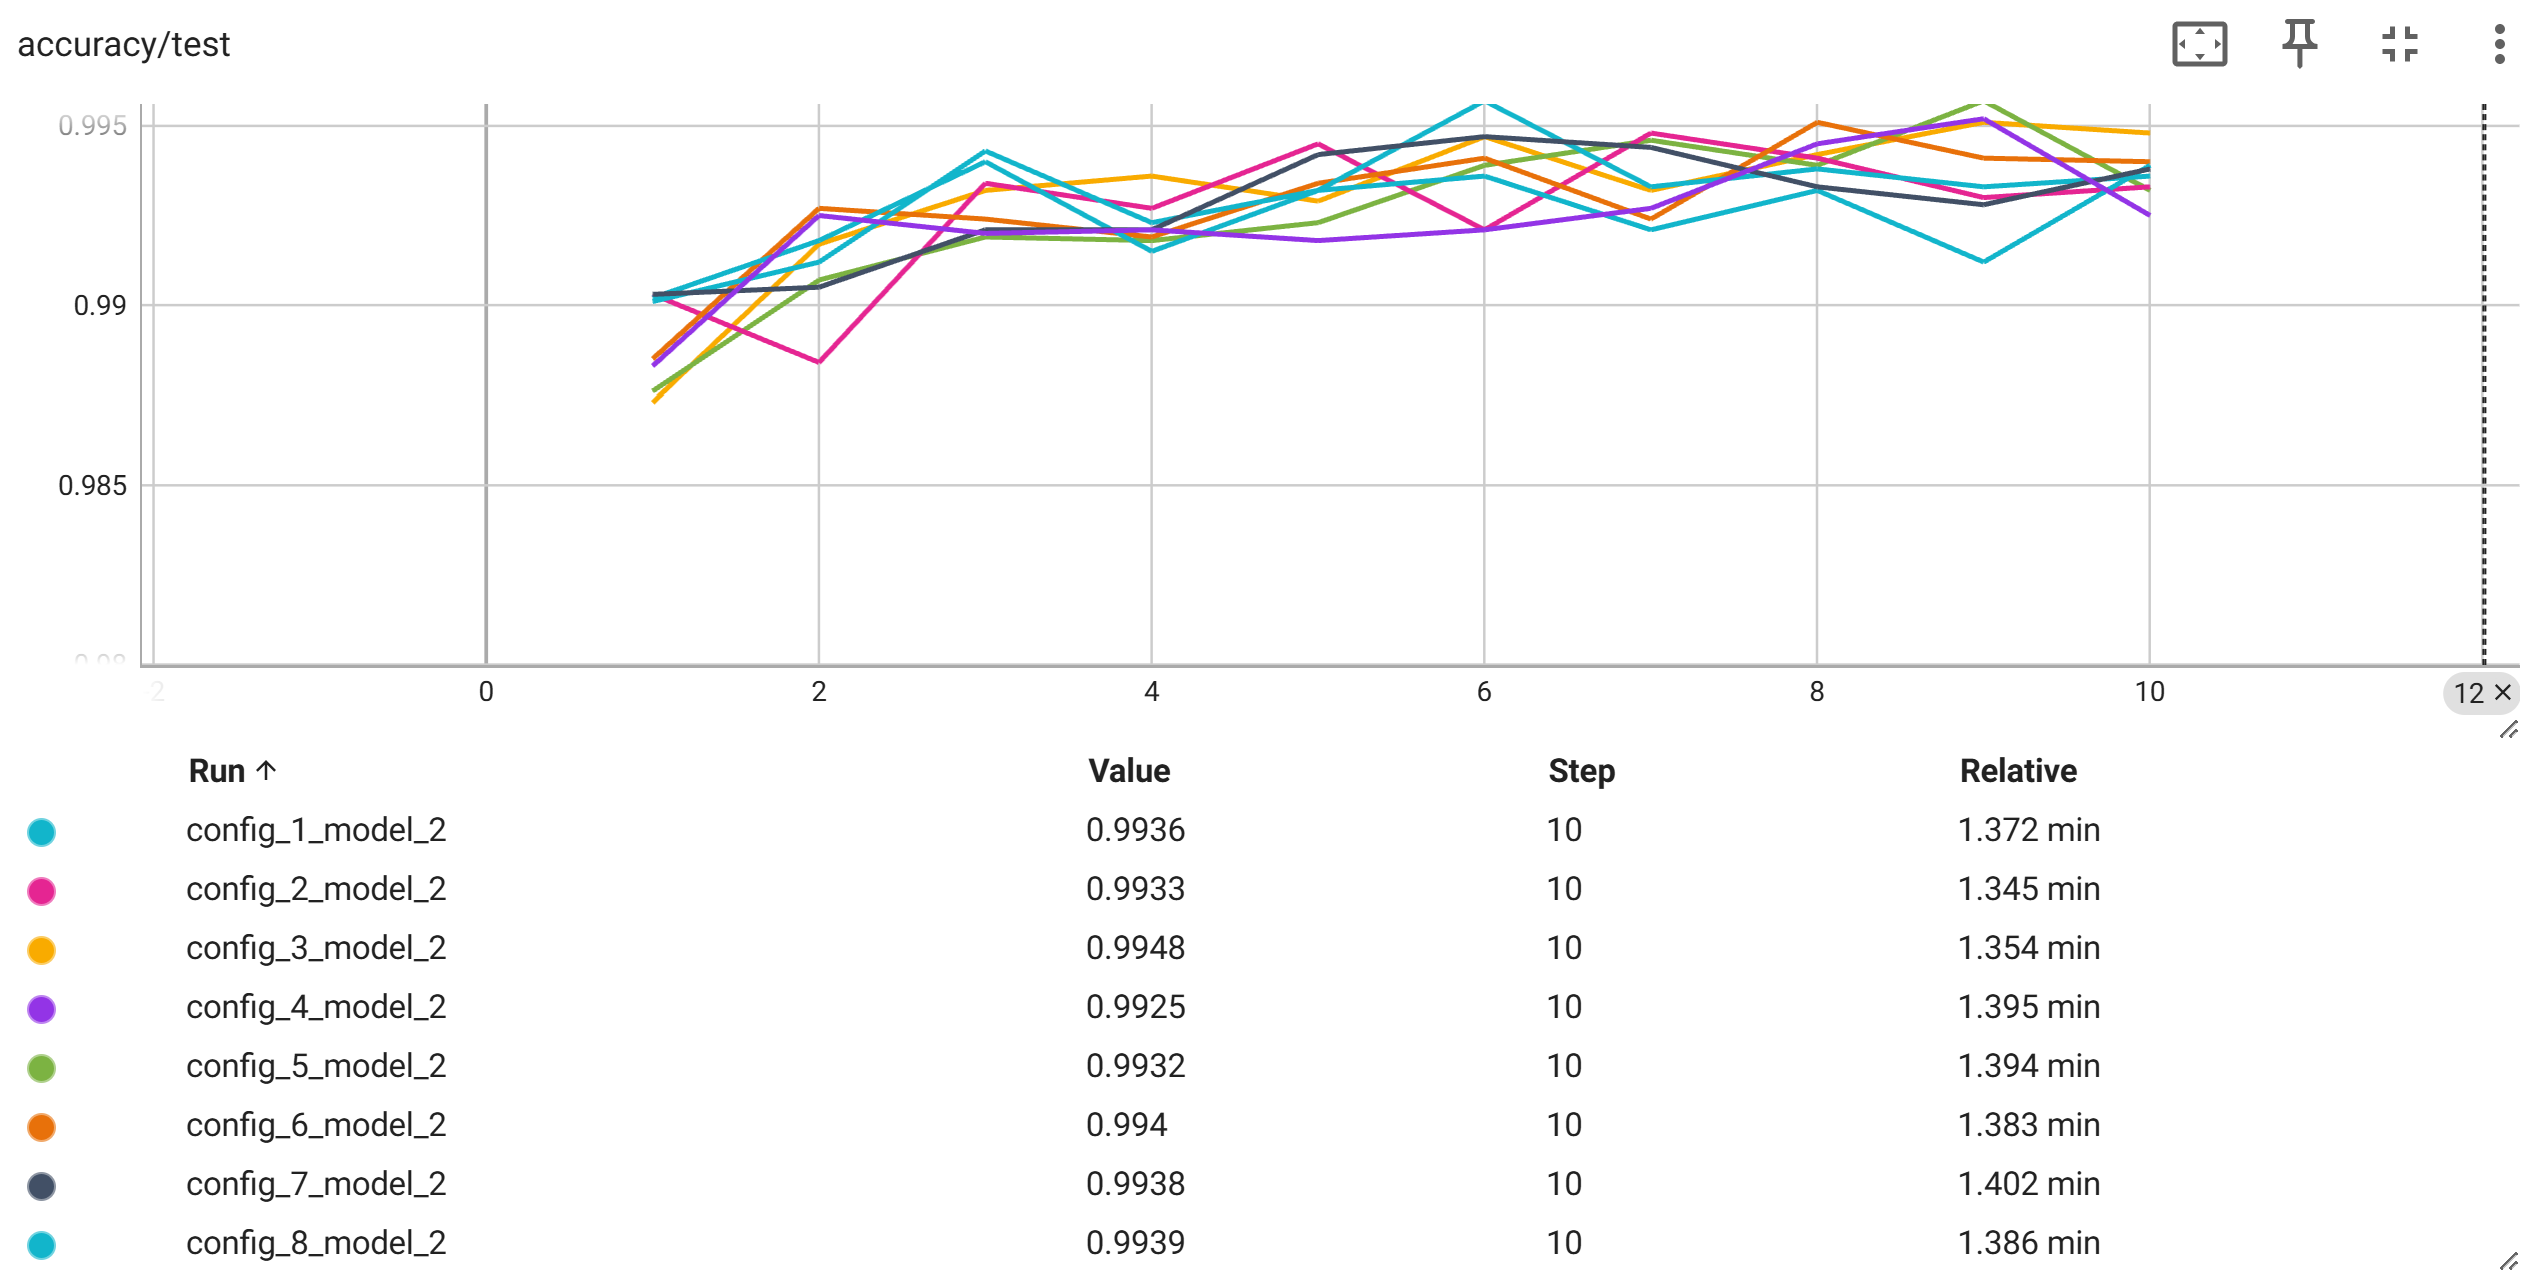
\includegraphics[width=\textwidth]{src/model_2_test_accurary.png}
        \caption{测试准确率}
        \label{fig:deep_test_acc}
    \end{subfigure}
    \caption{深层 CNN（五卷积层 + 批量归一化结构）在 8 组超参数配置下的准确率曲线。
    图例标签与超参数配置的对应关系见表~\ref{tab:legend_mapping}。}
    \label{fig:deep_cnn_accuracy}
\end{figure}

从图中可以观察到：
\begin{enumerate}
    \item 深层网络的训练准确率收敛速度明显快于基础网络：在首个训练轮次结束时，
          深层网络的训练准确率已达到约 97\% 以上，而基础网络仅达到约 92\%--94\%；
    \item 深层网络的测试准确率曲线更为平稳，不同超参数配置间的差异较小，
          再次印证了其对超参数变化具有较强的鲁棒性；
    \item 基础网络在训练准确率上存在较明显的配置间差异，尤其是使用较高学习率（0.001）时，
          收敛速度明显慢于低学习率（0.0005）的配置；
    \item 两种模型的测试准确率均未出现明显的过拟合迹象（训练准确率与测试准确率未出现显著背离），
          说明模型容量与数据集规模匹配良好。
\end{enumerate}

\section{调试与错误排查}

本实验在代码中实现了完善的日志记录机制，便于调试与错误排查。
调试信息通过两种方式记录：

\begin{enumerate}
    \item \textbf{文本日志}：使用 Python 标准库 \texttt{logging} 模块，为每个实验运行创建独立的日志文件。
          日志包含实验启动信息（模型名称、配置文件路径、日志路径）、
          每个训练轮次的训练损失、训练准确率、测试损失和测试准确率、以及最终的最佳准确率和模型保存路径。
          所有日志文件存储在 \texttt{logs/} 目录下，
          文件命名格式为 \texttt{config\_\{i\}\_model\_\{j\}.log}
          （其中 $i\in\{1,\dots,8\}$ 对应超参数组合编号，$j=1$ 对应基础 CNN，$j=2$ 对应深层 CNN）。

    \item \textbf{TensorBoard 可视化}：使用 PyTorch 的 \texttt{SummaryWriter} 将训练过程中的标量指标
          （批次级训练损失、训练轮次级训练损失、训练准确率、测试损失、测试准确率）
          实时写入 TensorBoard 事件文件，存储在 \texttt{runs/} 目录下。
          可通过 \texttt{tensorboard --logdir=runs} 命令启动可视化面板，
          直观对比不同实验的训练曲线。
\end{enumerate}

在实际运行过程中，如果实验出现错误（例如中途崩溃、GPU 内存不足、数据加载异常等），
可以通过以下方式进行排查：
\begin{itemize}
    \item 查看对应日志文件中的错误信息和最后一条记录，确定崩溃发生的训练轮次和批次位置；
    \item 检查 TensorBoard 中的损失曲线是否出现异常（如突然飙升或变为 NaN），判断是否存在梯度爆炸等问题；
    \item 验证模型检查点（\texttt{model/*.pth}）是否完整保存，若训练提前中断，可从最近的检查点恢复。
\end{itemize}

这一日志系统确保了实验的可追溯性和可复现性，是深度学习工程实践中的重要组成部分。

\section{结论}

本实验通过在 MNIST 手写数字识别任务上对两种卷积神经网络架构和八种超参数配置进行系统对比，得出以下结论：

\begin{enumerate}
    \item \textbf{深层网络显著提升性能}：引入批量归一化的五卷积层深层网络在所有超参数配置下均优于双卷积层基础网络，
          最佳准确率达到 99.57\%，相比基础网络的 99.37\% 有显著提升；
    \item \textbf{低学习率表现更优}：当学习率为 0.0005 时，两种模型的整体表现均优于学习率为 0.001 时；
    \item \textbf{批量归一化提供隐含正则化}：深层网络在不使用权重衰减时表现最佳，
          说明批量归一化本身已具备一定的正则化效果，额外的权重衰减可能限制模型容量；
    \item \textbf{网格搜索是有效的超参数调优方法}：通过 $2\times2\times2$ 的网格搜索，
          成功定位了各模型的最优超参数组合。
\end{enumerate}

未来的工作可以进一步探索数据增强策略、学习率调度器以及更现代的网络结构（如残差连接）对性能的影响。

\appendix
\section{附录：完整代码}

本项目的完整代码结构如下：

\begin{verbatim}
CNN-MNIST/
├── model.py              # 模型定义（基础 CNN 与深层 CNN）
├── dataloader.py         # 数据加载与预处理
├── train.py              # 训练与评估循环
├── main.py               # 主入口，解析配置、训练、保存
├── log.py                # 日志配置
├── predict_handwritten.py # 自定义手写数字预测
├── run_experiments.sh    # 批量实验脚本
├── config/               # 16 个 YAML 配置文件
├── logs/                 # 训练日志输出
├── model/                # 保存的模型检查点
├── runs/                 # TensorBoard 事件文件
├── numbersbyHAND/        # 手写数字测试图像
├── src/                  # TensorBoard 截图等素材
└── report.tex            # 本报告 LaTeX 源文件
\end{verbatim}

\subsection{model.py —— 模型定义}

\lstinputlisting[language=Python, caption=model.py]{model.py}

\subsection{dataloader.py —— 数据加载}

\lstinputlisting[language=Python, caption=dataloader.py]{dataloader.py}

\subsection{train.py —— 训练与评估}

\lstinputlisting[language=Python, caption=train.py]{train.py}

\subsection{main.py —— 主程序入口}

\lstinputlisting[language=Python, caption=main.py]{main.py}

\subsection{log.py —— 日志模块}

\lstinputlisting[language=Python, caption=log.py]{log.py}

\subsection{predict\_handwritten.py —— 手写数字预测}

\lstinputlisting[language=Python, caption=predict\_handwritten.py]{predict\_handwritten.py}

\subsection{run\_experiments.sh —— 批量实验脚本}

\lstinputlisting[language=bash, caption=run\_experiments.sh]{run\_experiments.sh}

\end{document}
